\section{Capa física: numerología y recursos}\label{sec:numerologia}

\subsection{Numerología: \texorpdfstring{$\mu$}{mu}, SCS, slots y símbolos}
A diferencia del LTE convencional, que usa para los datos una única separación entre subportadoras de 15~kHz, NR admite una familia de numerologías escaladas por potencias de dos \cite[§4.2]{ts38211}:
\begin{equation}
\Delta f = 2^{\mu}\cdot 15~\text{kHz}, \qquad \mu \in \{0,1,2,3,4\}.
\label{eq:scs}
\end{equation}
La trama dura siempre 10~ms y se divide en 10 subtramas de 1~ms. Cada subtrama tiene $2^\mu$ slots, y cada slot, 14 símbolos OFDM con CP normal \cite[§4.3.1, tabla~4.3.2-1]{ts38211}. Por lo tanto, al duplicar la SCS se reduce a la mitad la duración del símbolo y del slot (\cref{tab:numerologia}).

\begin{table}[htbp]
\centering
\caption{Numerologías de NR con CP normal (TS~38.211, tablas 4.2-1 y 4.3.2-1). La duración del CP es la de los símbolos comunes; el primero de cada medio subtrama tiene $16\kappa T_c = 0{,}52~\mu$s más.}
\label{tab:numerologia}
\begin{tabular}{cccccc}
\toprule
$\mu$ & $\Delta f$ [kHz] & slots/trama & slot [ms] & símbolo útil [$\mu$s] & CP [$\mu$s] \\
\midrule
0 & 15 & 10 & 1 & 66,67 & 4,69 \\
\rowcolor{azul!10} 1 & 30 & 20 & 0,5 & 33,33 & 2,34 \\
2 & 60 & 40 & 0,25 & 16,67 & 1,17 \\
3 & 120 & 80 & 0,125 & 8,33 & 0,59 \\
4 & 240 & 160 & 0,0625 & 4,17 & 0,29 \\
\bottomrule
\end{tabular}
\end{table}

La celda n78 usa $\mu=1$ (30~kHz): un slot dura 0,5~ms y hay 20 slots por trama. El símbolo útil dura $T_u = 1/\Delta f = 33{,}33~\mu$s. La celda n3 usa $\mu=0$, como LTE.

La elección de la numerología es un compromiso: una SCS mayor acorta el símbolo, lo que reduce la latencia y da más tolerancia al Doppler y al ruido de fase, pero también acorta el CP, lo que reduce la tolerancia al ensanchamiento temporal del canal (\cref{sec:cp}). En n78, 30~kHz es el valor típico de banda media.

\subsection{Unidad de tiempo \texorpdfstring{$T_c$}{Tc} y frecuencia de muestreo}\label{sec:fs}
TS~38.211 define todas las duraciones como múltiplos de una unidad básica \cite[§4.1]{ts38211}:
\begin{equation}
T_c = \frac{1}{\Delta f_\text{max}\cdot N_f} = \frac{1}{480\cdot 10^3~\text{Hz}\cdot 4096} \approx 0{,}509~\text{ns},
\label{eq:tc}
\end{equation}
que corresponde a la mayor SCS prevista (480~kHz) con una FFT de 4096 puntos. La relación con la unidad de LTE, $T_s = 1/(15~\text{kHz}\cdot 2048) = 32{,}55$~ns, es la constante
\begin{equation}
\kappa = \frac{T_s}{T_c} = 64.
\label{eq:kappa}
\end{equation}
La ``frecuencia de muestreo básica'' de NR es entonces $1/T_c = 1{,}966\,08$~GHz. \textbf{No es la frecuencia a la que muestrea un equipo real:} es una grilla temporal común que permite escribir todas las duraciones de todas las numerologías como números enteros. Un transmisor real muestrea a
\begin{equation}
f_s = N_\text{FFT}\cdot \Delta f,
\label{eq:fs}
\end{equation}
donde $N_\text{FFT}$ es el tamaño de la IFFT/FFT elegido por la implementación. La condición básica es que $N_\text{FFT}$ sea mayor que la cantidad de subportadoras ocupadas, para que la señal compleja en banda base quepa en $[-f_s/2, f_s/2)$ con margen para los filtros; en la práctica también influyen los relojes que admite el hardware y el costo de la FFT.

\paragraph{Frecuencia de muestreo de la celda.} La B210 se configuró a $f_s = 23{,}04$~MS/s:
\begin{equation}
f_s = 1536\cdot 15~\text{kHz} = 768\cdot 30~\text{kHz} = 23{,}04~\text{MHz}.
\label{eq:fs_celda}
\end{equation}
\begin{itemize}
  \item En n78 ($\Delta f = 30$~kHz) la FFT es de 768 puntos, y en n3 ($\Delta f=15$~kHz), de 1536 puntos. En ambos casos, el ancho de banda de muestreo es el mismo: $1536\times 15~\text{kHz}$.
  \item Hay 612 subportadoras ocupadas en n78 (51~PRB $\times$ 12) y 1272 en n3 (106~PRB $\times$ 12): ambas entran en la FFT, con un factor de sobremuestreo de $768/612 \approx 1{,}25$ y $1536/1272\approx 1{,}21$.
  \item $768 = 2^8\cdot 3$ y $1536 = 2^9\cdot 3$ no son potencias de dos, pero se calculan eficientemente con FFT de base mixta. La alternativa de potencia de dos inmediata (1024 puntos a 30~kHz) exige 30,72~MS/s.
  \item 23,04~MS/s es una elección compatible y eficiente para 20~MHz en esta plataforma, no un mínimo universal. Con el formato \texttt{sc12} (12 bits por componente, 3 bytes por muestra compleja) el flujo es de $23{,}04\cdot 10^6\cdot 3 \approx 69$~MB/s en cada sentido. Ese caudal solo es sostenible por USB~3.0, lo que explica el primer problema práctico de la \cref{sec:crono}.
\end{itemize}

\Cref{tab:fs} compara las frecuencias de muestreo posibles para $\mu=1$. Las duraciones en muestras salen de multiplicar las de la norma ($2048\kappa 2^{-\mu} = 65\,536$, $144\kappa 2^{-\mu} = 4608$ y $144\kappa 2^{-\mu}+16\kappa = 5632$, en unidades de $T_c$) por $f_s T_c$. Por ejemplo, a 23,04~MS/s, $f_s T_c = 23{,}04/1966{,}08 = 3/256$.

\begin{table}[htbp]
\centering
\caption{Muestras por símbolo y por slot para $\mu=1$ según la frecuencia de muestreo. En todas, un slot dura 0,5~ms.}
\label{tab:fs}
\begin{tabular}{lcccc}
\toprule
$f_s$ & $N_\text{FFT}$ & CP normal & CP largo (1.\textsuperscript{er} símbolo) & muestras por slot \\
\midrule
\rowcolor{azul!10} 23,04 MS/s (usada) & 768 & 54 & 66 & $768\cdot14+54\cdot13+66 = 11\,520$ \\
30,72 MS/s & 1024 & 72 & 88 & 15\,360 \\
61,44 MS/s & 2048 & 144 & 176 & 30\,720 \\
1,966 GHz ($1/T_c$) & 65\,536 & 4608 & 5632 & 983\,040 \\
\bottomrule
\end{tabular}
\end{table}

La comprobación para la frecuencia usada es directa: $11\,520 / 23{,}04~\text{MS/s} = 0{,}5$~ms. El CP vale $54/23{,}04~\text{MHz} = 2{,}344~\mu$s y el largo, $66/23{,}04~\text{MHz} = 2{,}865~\mu$s, idénticos a los de TS~38.211.

\subsection{Grilla de recursos, RE y PRB}
El recurso elemental es el \textbf{resource element} (RE): una subportadora durante un símbolo OFDM. Un \textbf{PRB} agrupa 12 subportadoras consecutivas en frecuencia \cite[§4.4]{ts38211}. A diferencia de LTE, en NR el PRB se define solo en frecuencia: en el tiempo, la unidad de planificación es el slot o una fracción de él (asignaciones de 2 a 14 símbolos). Con $\mu=1$, un PRB ocupa $12\cdot 30 = 360$~kHz.

Todas las grillas se referencian al \textbf{punto A}, una frecuencia común a todas las numerologías. A partir de él se numeran los CRB (\emph{common resource blocks}), y una \emph{bandwidth part} (BWP) es un subconjunto contiguo de CRB con una numerología dada. En esta celda hay una sola BWP, que ocupa los 51~PRB del canal.

\subsection{Cálculo de PRB y de banda de guarda}\label{sec:guarda}
TS~38.101-1 fija, para cada ancho de banda de canal y SCS, la cantidad máxima de PRB $N_\text{RB}$ (tabla~5.3.2-1) y la banda de guarda mínima a cada lado (tabla~5.3.3-1) \cite{ts38101}\verif. La banda de guarda mínima se obtiene de
\begin{equation}
G_\text{BW} = \frac{\text{BW}_\text{canal} - N_\text{RB}\cdot 12\cdot\Delta f}{2} - \frac{\Delta f}{2},
\label{eq:guarda}
\end{equation}
donde el término $\Delta f/2$ tiene en cuenta que la grilla de subportadoras está desplazada media subportadora respecto del centro del canal.

\paragraph{n78, 20~MHz, 30~kHz ($N_\text{RB}=51$).}
\begin{align}
\text{BW ocupado} &= 51\cdot 12\cdot 30~\text{kHz} = 18\,360~\text{kHz} \quad (91{,}8~\%\text{ del canal}),\\
G_\text{BW} &= \frac{20\,000-18\,360}{2} - \frac{30}{2} = 820 - 15 = 805~\text{kHz}.
\end{align}

\paragraph{n3, 20~MHz, 15~kHz ($N_\text{RB}=106$).}
\begin{align}
\text{BW ocupado} &= 106\cdot 12\cdot 15~\text{kHz} = 19\,080~\text{kHz} \quad (95{,}4~\%),\\
G_\text{BW} &= \frac{20\,000-19\,080}{2} - 7{,}5 = 460 - 7{,}5 = 452{,}5~\text{kHz}.
\end{align}

Con 15~kHz se aprovecha mejor el canal (95,4~\% contra 91,8~\%) porque la guarda que necesitan los filtros es, en proporción, menor. LTE, con 100~PRB en 20~MHz, ocupaba solo el 90~\%. La guarda protege a los canales adyacentes de la emisión fuera de banda: los lóbulos laterales de las subportadoras OFDM decaen lentamente (como una sinc) y el filtrado o el \emph{windowing} necesita una banda de transición.

\subsection{Prefijo cíclico}\label{sec:cp}
\subsubsection{Función del CP}
El canal multitrayecto tiene una respuesta al impulso de duración $\tau_\text{max}$ (\emph{delay spread}). Si se antepone a cada símbolo una copia de sus últimas $N_\text{CP}$ muestras, con $T_\text{CP}\ge\tau_\text{max}$:
\begin{enumerate}
  \item la interferencia entre símbolos (ISI) queda confinada al CP, que el receptor descarta;
  \item la convolución lineal con el canal se vuelve \textbf{circular} dentro de la ventana de la FFT, así que cada subportadora ve una ganancia compleja $H_k$ y se ecualiza con un solo coeficiente, sin interferencia entre portadoras (ICI).
\end{enumerate}
Por eso, \textbf{el valor mínimo del prefijo cíclico es el delay spread del canal} (más el error residual de sincronización):
\begin{equation}
T_\text{CP} \ge \tau_\text{max}.
\label{eq:cpmin}
\end{equation}
El costo es la eficiencia: el CP no lleva información nueva, así que se pierde una fracción $T_\text{CP}/(T_u + T_\text{CP})$ del tiempo y de la energía.

\subsubsection{Ejercicio planteado por la cátedra}\label{sec:ejercicio_cp}
Se supone un delay spread igual a un cuarto del símbolo útil, con $\Delta f=15$~kHz:
\begin{equation}
\tau = \frac{1}{4\,\Delta f} = \frac{1}{4\cdot 15~\text{kHz}} = 16{,}67~\mu\text{s}.
\end{equation}
Con $f_s = 1536\cdot 15~\text{kHz} = 23{,}04$~MHz, el período de muestreo es
\begin{equation}
T_s = \frac{1}{f_s} = \frac{1}{23{,}04~\text{MHz}} = 43{,}40~\text{ns},
\end{equation}
y el CP necesario, en muestras,
\begin{equation}
N_\text{CP} = \frac{\tau}{T_s} = \frac{16{,}67~\mu\text{s}}{43{,}40~\text{ns}} = 384~\text{muestras}.
\end{equation}
Sumadas a las 1536 muestras de la IFFT, el símbolo completo tiene $1536+384 = 1920$ muestras, y dura
\begin{equation}
T_\text{símb} = \frac{1920}{23{,}04~\text{MHz}} = 83{,}33~\mu\text{s} = 66{,}67~\mu\text{s (útil)} + 16{,}67~\mu\text{s (CP)}.
\end{equation}
Con una IFFT de 2048 puntos ($f_s = 30{,}72$~MHz) el CP sería de 512 muestras: cambia la cantidad de muestras, pero no la duración del símbolo, que depende solo de $\Delta f$ y de la fracción de CP. Catorce símbolos de este tipo duran $14\cdot 83{,}33~\mu\text{s} = 1{,}167$~ms.

\subsubsection{Comparación con NR}
Con un CP de $T_u/4$ no entran 14 símbolos en 1~ms, sino
\begin{equation}
\left\lfloor \frac{1~\text{ms}}{83{,}33~\mu\text{s}} \right\rfloor = 12~\text{símbolos}.
\end{equation}
Ese es exactamente el caso del \textbf{CP extendido}: en LTE, $512$ muestras a 30,72~MHz (16,67~$\mu$s) y 12 símbolos por subtrama. En NR, el CP extendido solo existe para $\mu=2$ ($512\kappa 2^{-\mu}T_c$) \cite[§5.3.1]{ts38211}.

El \textbf{CP normal} de NR es mucho más corto. Según TS~38.211 §5.3.1,
\begin{equation}
N_{\text{CP},l}^{\mu} =
\begin{cases}
144\kappa\, 2^{-\mu} + 16\kappa & l = 0 \text{ o } l = 7\cdot 2^{\mu}\\
144\kappa\, 2^{-\mu} & \text{en otro caso}
\end{cases}
\qquad[\text{en unidades de } T_c].
\label{eq:ncp}
\end{equation}
Para $\mu=0$, a 30,72~MHz, son 144 muestras (4,69~$\mu$s), y 160 en el primer símbolo de cada medio subframe. Así entran 14 símbolos en 1~ms:
\begin{equation}
2048\cdot 14 + 144\cdot 14 + 16\cdot 2 = 28\,672 + 2016 + 32 = 30\,720~\text{muestras} = 1~\text{ms}\times 30{,}72~\text{MS/s}.
\end{equation}
Para la celda n3, a 23,04~MHz con FFT de 1536, la misma cuenta da $1536\cdot 14 + 108\cdot 14 + 12\cdot 2 = 23\,040$ muestras. Para la celda n78 ($\mu=1$), el CP normal es de $144\cdot 64\cdot 2^{-1}\,T_c = 2{,}344~\mu$s, y de $2{,}865~\mu$s en el primer símbolo de cada slot.

\textbf{Importante:} en NR, los 14 símbolos forman un \textbf{slot}, no una trama. La trama dura siempre 10~ms; según la numerología contiene entre 10 y 160 slots (\cref{tab:numerologia}).

\paragraph{Delay spread tolerable.} Un CP de $2{,}344~\mu$s cubre trayectos que difieren hasta
\begin{equation}
\Delta d = c\cdot T_\text{CP} = 3\cdot 10^8~\text{m/s}\cdot 2{,}344\cdot 10^{-6}~\text{s} \approx 703~\text{m}.
\end{equation}
Es más que suficiente para una jaula de Faraday o un ambiente de interiores (delay spreads de decenas a cientos de nanosegundos), y razonable para microceldas urbanas. Con 15~kHz, el CP de 4,69~$\mu$s tolera $\approx 1{,}4$~km.

\subsection{Estructura TDD}\label{sec:tdd}
En TDD, el gNB difunde en el SIB1 el patrón de slots \texttt{tdd-UL-DL-ConfigurationCommon} \cite[§11.1]{ts38213}. En la celda n78, ese patrón tiene un período de 5~ms (10 slots) y es \texttt{DDDDDDSUUU} (\cref{fig:tdd}):
\begin{itemize}
  \item 6 slots de bajada (D);
  \item 1 slot especial (S) con 8 símbolos de bajada, 0 de subida y 6 de guarda;
  \item 3 slots de subida (U).
\end{itemize}
El \textbf{período de guarda} cubre el tiempo de conmutación del hardware y el retardo de ida y vuelta: el UE tiene que terminar de recibir la bajada y adelantar su transmisión en el \emph{timing advance} (\cref{sec:ta}) sin que la subida se superponga con la bajada siguiente.

\begin{figure}[htbp]
\centering
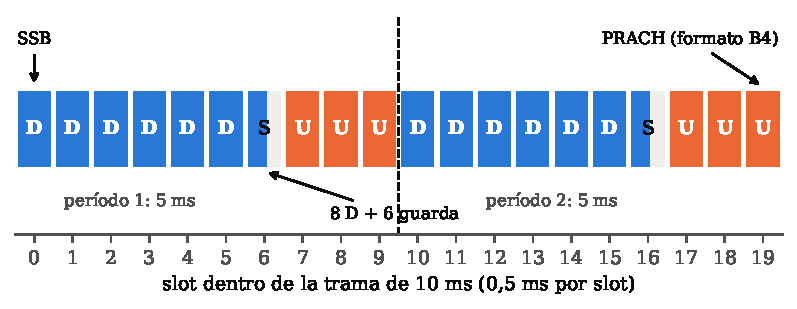
\includegraphics[width=\linewidth]{figuras/fig_tdd.pdf}
\caption{Patrón TDD de la celda n78 en una trama de 10~ms: dos períodos de 5~ms \texttt{DDDDDDSUUU}. El SSB va en el slot~0 y la ocasión de PRACH (formato B4, índice 159), en el slot~19.}
\label{fig:tdd}
\end{figure}

Las fracciones de símbolos por sentido en un período son:
\begin{align}
\text{DL:}\quad & \frac{6\cdot 14 + 8}{10\cdot 14} = \frac{92}{140} = 0{,}657, \label{eq:fdl}\\
\text{UL:}\quad & \frac{3\cdot 14}{140} = \frac{42}{140} = 0{,}30, \label{eq:ful}\\
\text{guarda:}\quad & \frac{6}{140} = 0{,}043.
\end{align}
Estas fracciones limitan el throughput de cada sentido (\cref{sec:tput}) y fijan cuánto hay que esperar un slot de subida (\cref{sec:latencia}).
